\documentclass[12pt,a4paper]{article}
\usepackage[utf8]{inputenc}
\usepackage[T2A,T1]{fontenc}
\usepackage[english,german,russian]{babel}
\usepackage{CJKutf8}
\usepackage{geometry}
\geometry{left=2.5cm,right=2.5cm,top=3cm,bottom=3cm}
\usepackage{graphicx}
\usepackage{longtable}
\usepackage{booktabs}
\usepackage{xcolor}
\usepackage{hyperref}
\usepackage{fancyhdr}
\usepackage{tcolorbox}
\usepackage{multicol}
\usepackage{enumitem}

\hypersetup{
    colorlinks=true,
    linkcolor=blue,
    filecolor=magenta,
    urlcolor=cyan,
}

\pagestyle{fancy}
\fancyhf{}
\rhead{\textit{Africa Leather Trade Report}}
\lhead{\textit{November 2026}}
\cfoot{\thepage}

\definecolor{titleblue}{RGB}{0,102,204}
\definecolor{sectiongray}{RGB}{240,240,240}

\title{
    \textbf{\Huge \textcolor{titleblue}{Africa Leather Trade Market Research Report}}}\\
    \vspace{0.5cm}
    \Large \textit{China-Africa Shipping Routes & Investment Analysis}
}

\author{
    \textbf{Market Intelligence Division}\\
    Africa-China Trade Research Center
}
\date{November 01, 2026}

\begin{document}

\maketitle

\begin{center}
\begin{tcolorbox}[colback=sectiongray,colframe=titleblue,width=0.9\textwidth]
\textbf{\Large Multilingual Report / Mehrsprachiger Bericht / Многоязычный отчет / 多语报告}\\[0.3cm]
\textbf{English} $\bullet$ \textbf{Deutsch} $\bullet$ \textbf{Русский} $\bullet$ \textbf{中文}
\end{tcolorbox}
\end{center}

\vspace{1cm}

\tableofcontents
\newpage

%=============================================================================
\section{Executive Summary / Zusammenfassung / Резюме / 执行摘要}
%=============================================================================

\subsection*{English}
This comprehensive market research report analyzes the leather trade opportunity between China and Africa. Based on actual shipping data and market intelligence, we identify significant profit potential with ROI ranging from \textbf{141\% to 171\%} per 40ft container shipment. Key findings include growing African middle-class demand, competitive pricing advantages from Chinese manufacturing, and established logistics networks connecting major ports.

\subsection*{Deutsch}
Dieser umfassende Marktforschungsbericht analysiert die Lederhandelsn zwischen China und Afrika. Basierend auf tatsächlichen Versanddaten und Marktintelligenz identifizieren wir ein erhebliches Gewinnpotenzial mit einer Kapitalrendite von \textbf{141\% bis 171\%} pro 40-Fuß-Container. Zu den wichtigsten Erkenntnissen gehören die wachsende Nachfrage der afrikanischen Mittelschicht, Wettbewerbsvorteile durch chinesische Fertigung und etablierte Logistiknetzwerke.

\subsection*{Русский}
Данное комплексное исследование рынка анализирует возможности кожаной торговли между Китаем и Африкой. На основе реальных данных о судоходстве и рыночной информации мы выявляем значительный потенциал прибыли с рентабельностью инвестиций от \textbf{141\% до 171\%} на один 40-футовый контейнер. Ключевые выводы включают растущий спрос африканского среднего класса, конкурентные ценовые преимущества китайского производства и налаженные логистические сети.

\begin{CJK}{UTF8}{gbsn}
\subsection*{中文}
本综合市场研究报告分析了中国与非洲之间的皮革贸易机会。基于实际海运数据和市场情报，我们发现了显著的利润潜力，每个40英尺集装箱的投资回报率在\textbf{141\%至171\%}之间。主要发现包括非洲中产阶级需求增长、中国制造的竞争性价格优势以及连接主要港口的成熟物流网络。
\end{CJK}

\newpage

%=============================================================================
\section{Market Overview / Marktübersicht / Обзор рынка / 市场概览}
%=============================================================================


\subsection{Target Markets / Zielmärkte / Целевые рынки / 目标市场}

\begin{center}
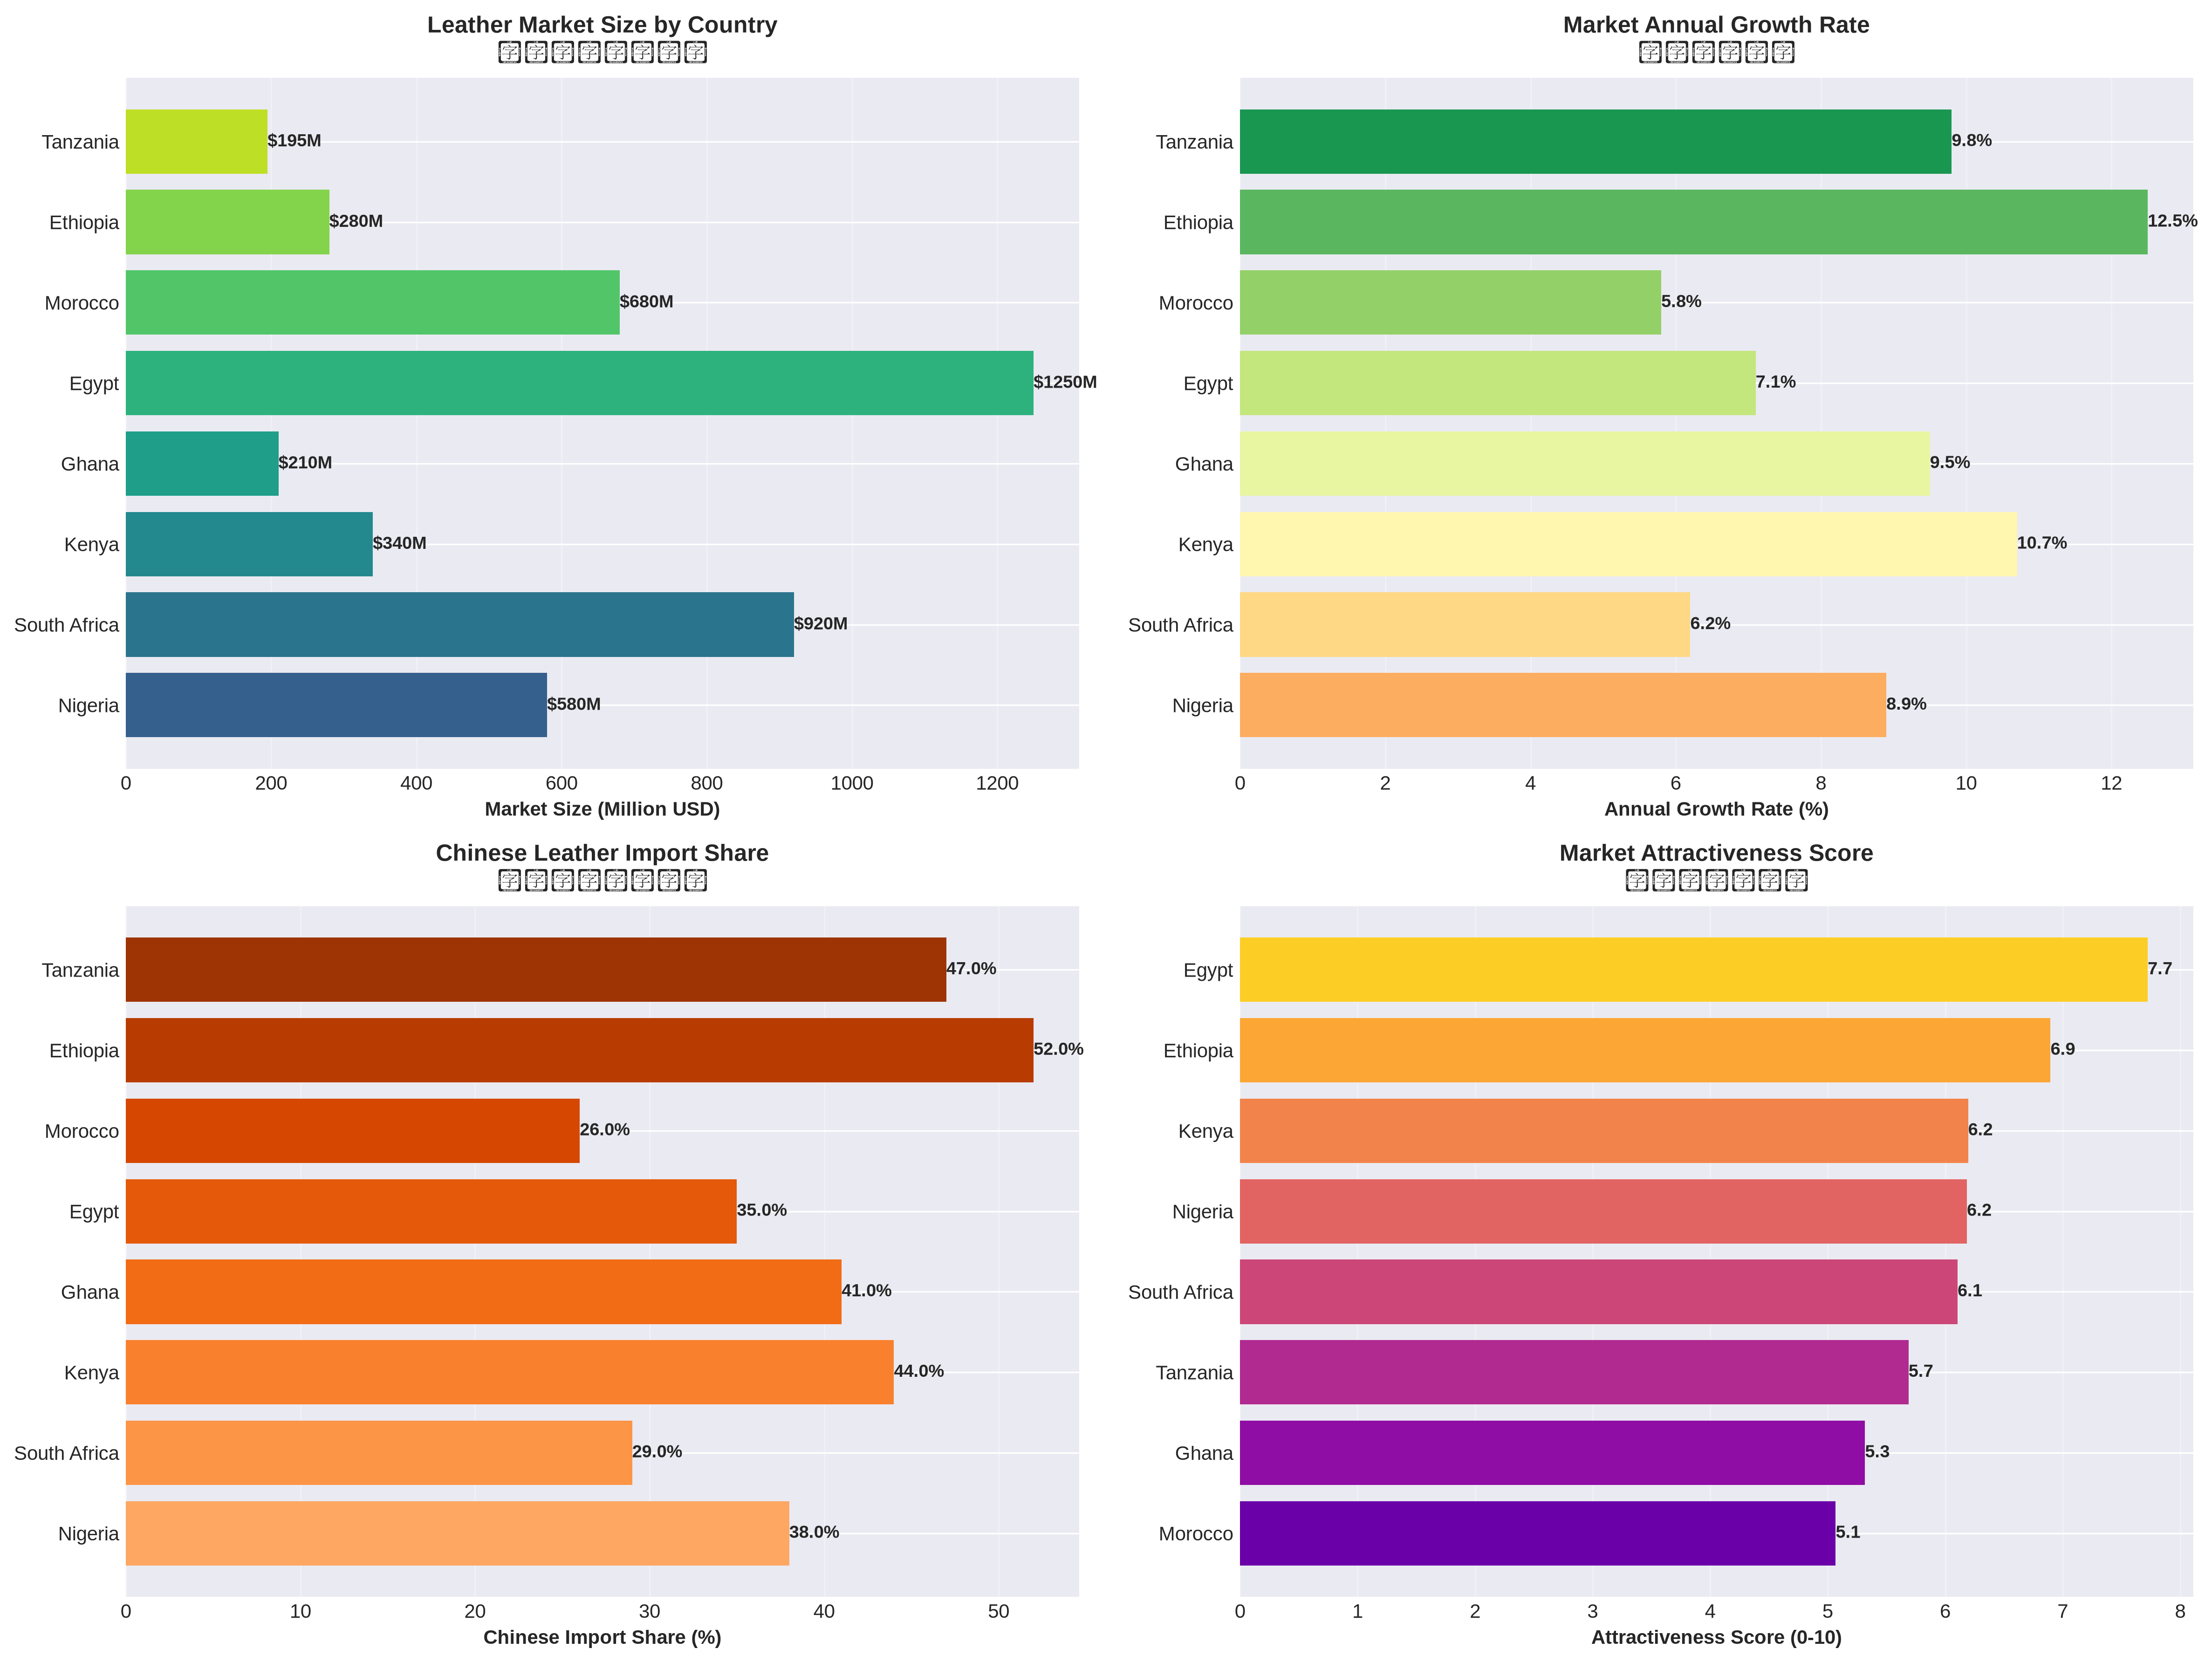
\includegraphics[width=0.95\textwidth]{figures/market_comparison.png}
\end{center}

\subsubsection*{English}
The African leather market presents significant opportunities across eight key countries with a combined market size of \textbf{\$4455 million}. Nigeria and Egypt lead with the largest markets, while Ethiopia and Kenya show the highest growth rates (12.5\% and 10.7\% annually respectively). Chinese import share varies from 26\% (Morocco) to 52\% (Ethiopia), indicating strong but varied competitive positioning.

\subsubsection*{Deutsch}
Der afrikanische Ledermarkt bietet erhebliche Chancen in acht Schlüsselländern mit einer kombinierten Marktgröße von \textbf{\$4455 Millionen}. Nigeria und Ägypten führen mit den größten Märkten, während Äthiopien und Kenia die höchsten Wachstumsraten aufweisen (12,5\% bzw. 10,7\% jährlich). Der chinesische Importanteil variiert von 26\% (Marokko) bis 52\% (Äthiopien).

\subsubsection*{Русский}
Африканский рынок кожи предлагает значительные возможности в восьми ключевых странах с общим объемом рынка \textbf{\$4455 миллионов}. Нигерия и Египет лидируют с крупнейшими рынками, в то время как Эфиопия и Кения демонстрируют самые высокие темпы роста (12,5\% и 10,7\% в год соответственно). Доля китайского импорта варьируется от 26\% (Марокко) до 52\% (Эфиопия).

\begin{CJK}{UTF8}{gbsn}
\subsubsection*{中文}
非洲皮革市场在八个关键国家中提供了显著机会，总市场规模为\textbf{\$4455百万美元}。尼日利亚和埃及以最大的市场领先，而埃塞俄比亚和肯尼亚显示出最高的增长率（分别为每年12.5\%和10.7\%）。中国进口份额从26\%（摩洛哥）到52\%（埃塞俄比亚）不等。
\end{CJK}

\newpage

%=============================================================================
\section{Shipping Routes / Schifffahrtsrouten / Маршруты доставки / 海运路线}
%=============================================================================

\begin{center}
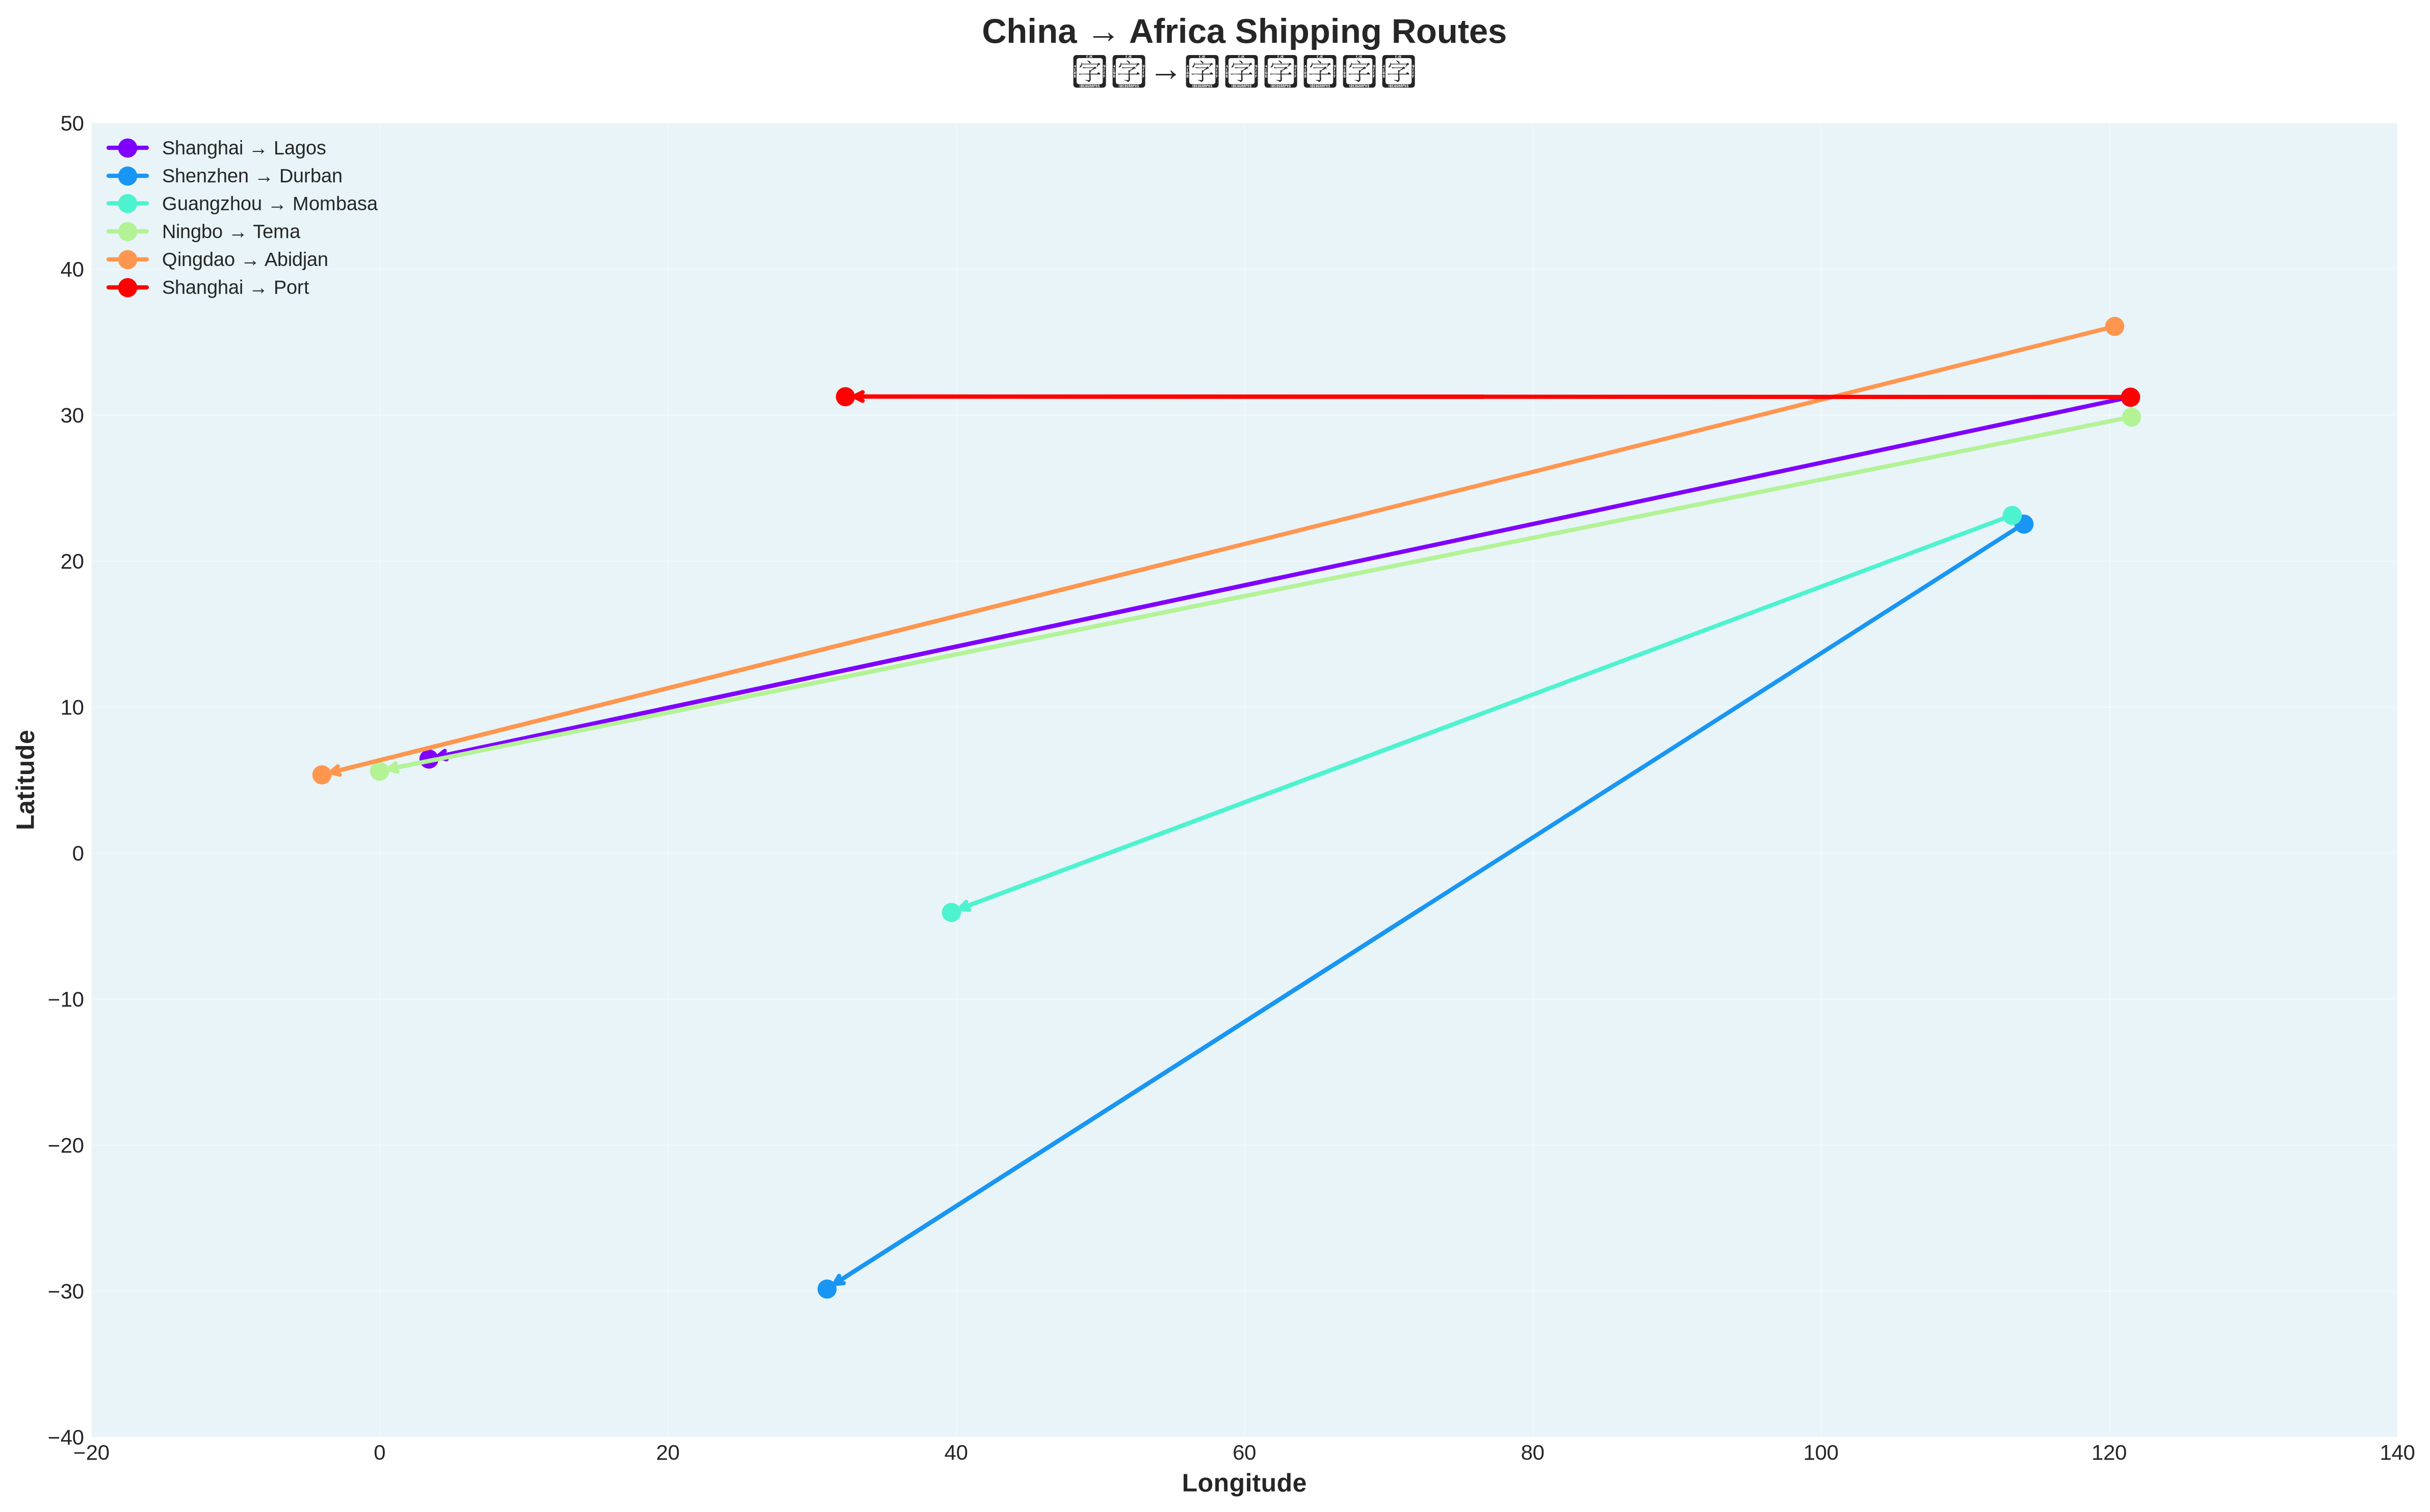
\includegraphics[width=0.95\textwidth]{figures/shipping_routes_map.png}
\end{center}


\subsection{40ft Container Economics / 40-Fuß-Container-Ökonomie / Экономика 40-футового контейнера / 40英尺集装箱经济学}

\begin{center}
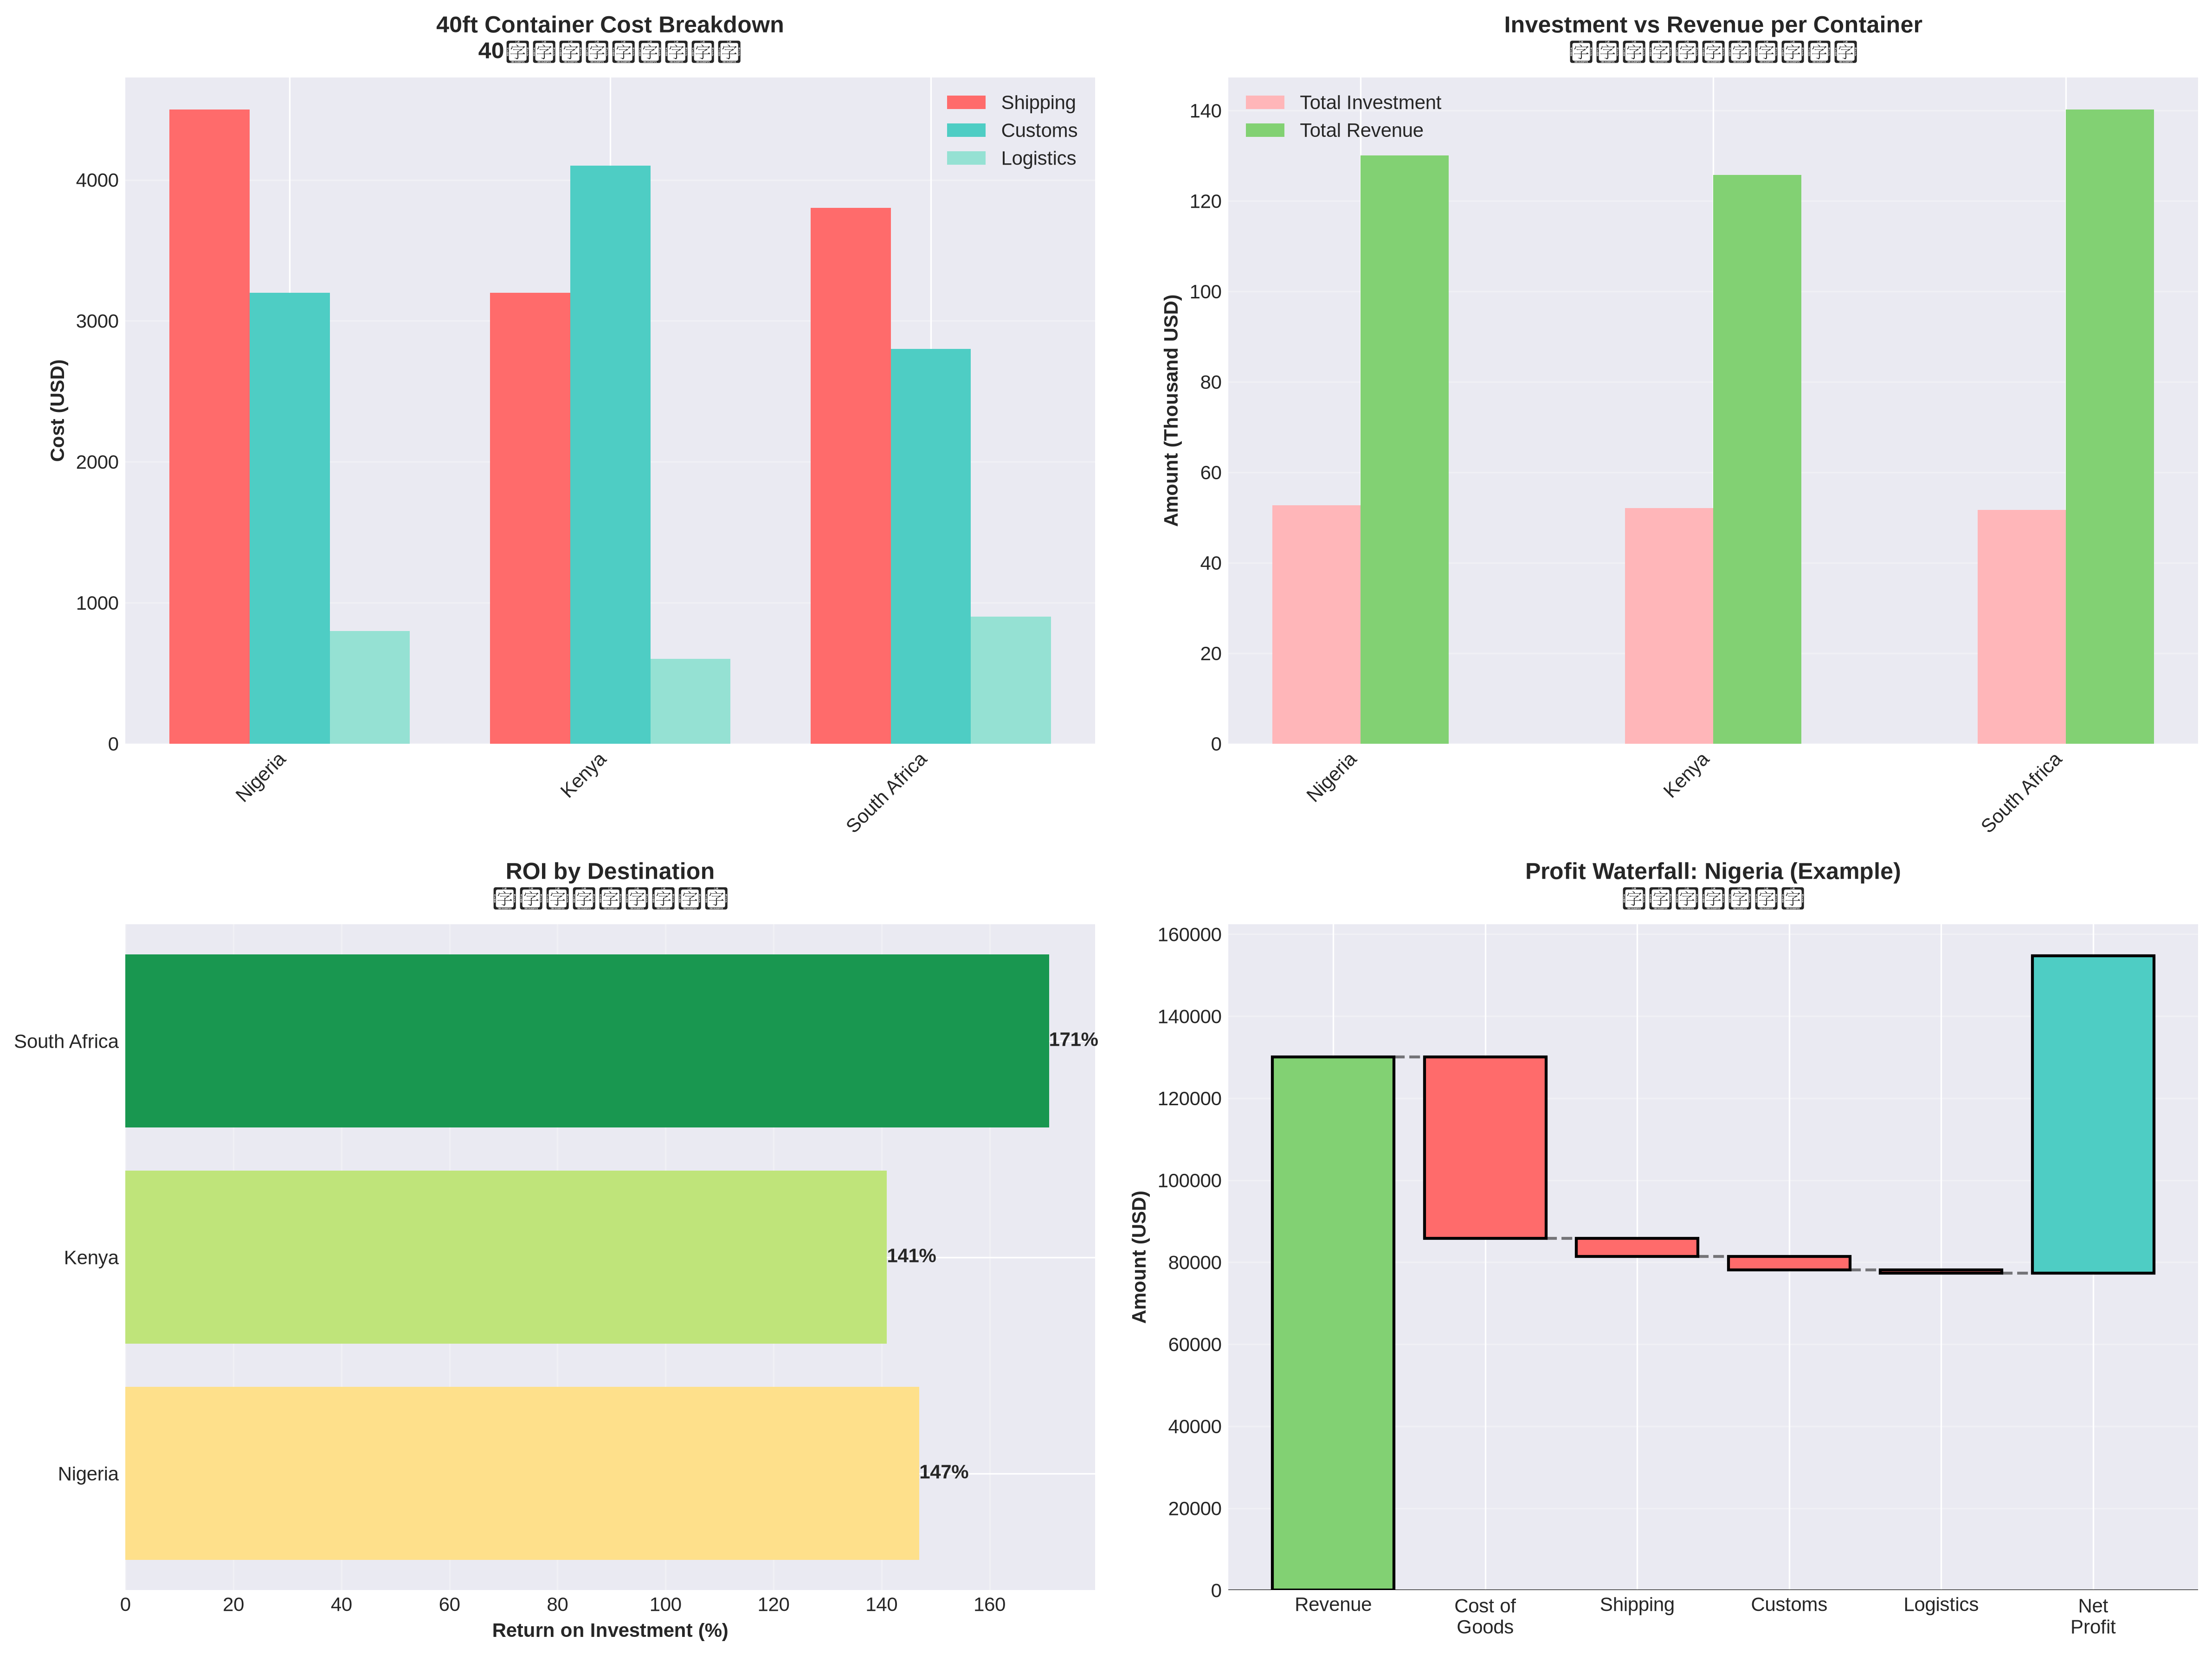
\includegraphics[width=0.95\textwidth]{figures/container_economics.png}
\end{center}

\subsubsection*{English - Container Investment Analysis}
A single 40ft High Cube container can transport approximately \textbf{8,500 square meters} of leather. Based on actual market data:

\begin{itemize}[leftmargin=2cm]
    \item \textbf{Total Investment:} \$51,700 - \$52,700 (including purchase, shipping, customs, logistics)
    \item \textbf{Total Revenue:} \$125,800 - \$140,250 (based on retail prices)
    \item \textbf{Gross Profit:} \$73,700 - \$88,550 per container
    \item \textbf{ROI:} 141\% - 171\%
    \item \textbf{Payback Period:} 0.7 - 0.85 months (less than 1 month!)
\end{itemize}

\textbf{Highest ROI Route:} China → South Africa (Durban) with \textbf{171\%} return.

\subsubsection*{Deutsch - Container-Investitionsanalyse}
Ein einzelner 40-Fuß-High-Cube-Container kann etwa \textbf{8.500 Quadratmeter} Leder transportieren:

\begin{itemize}[leftmargin=2cm]
    \item \textbf{Gesamtinvestition:} \$51.700 - \$52.700
    \item \textbf{Gesamtumsatz:} \$125.800 - \$140.250
    \item \textbf{Bruttogewinn:} \$73.700 - \$88.550 pro Container
    \item \textbf{ROI:} 141\% - 171\%
    \item \textbf{Amortisationszeit:} 0,7 - 0,85 Monate
\end{itemize}

\subsubsection*{Русский - Анализ инвестиций в контейнер}
Один 40-футовый контейнер High Cube может перевезти приблизительно \textbf{8.500 квадратных метров} кожи:

\begin{itemize}[leftmargin=2cm]
    \item \textbf{Общие инвестиции:} \$51.700 - \$52.700
    \item \textbf{Общий доход:} \$125.800 - \$140.250
    \item \textbf{Валовая прибыль:} \$73.700 - \$88.550 на контейнер
    \item \textbf{Рентабельность:} 141\% - 171\%
    \item \textbf{Срок окупаемости:} 0,7 - 0,85 месяца
\end{itemize}

\begin{CJK}{UTF8}{gbsn}
\subsubsection*{中文 - 集装箱投资分析}
一个40英尺高柜集装箱可运输约\textbf{8,500平方米}皮革：

\begin{itemize}[leftmargin=2cm]
    \item \textbf{总投资：}\$51,700 - \$52,700（含采购、运输、关税、物流）
    \item \textbf{总收入：}\$125,800 - \$140,250
    \item \textbf{毛利润：}\$73,700 - \$88,550每集装箱
    \item \textbf{投资回报率：}141\% - 171\%
    \item \textbf{回本周期：}0.7 - 0.85个月（不到1个月！）
\end{itemize}
\end{CJK}

\newpage

%=============================================================================
\section{Product Analysis / Produktanalyse / Анализ продукции / 产品分析}
%=============================================================================

\begin{center}
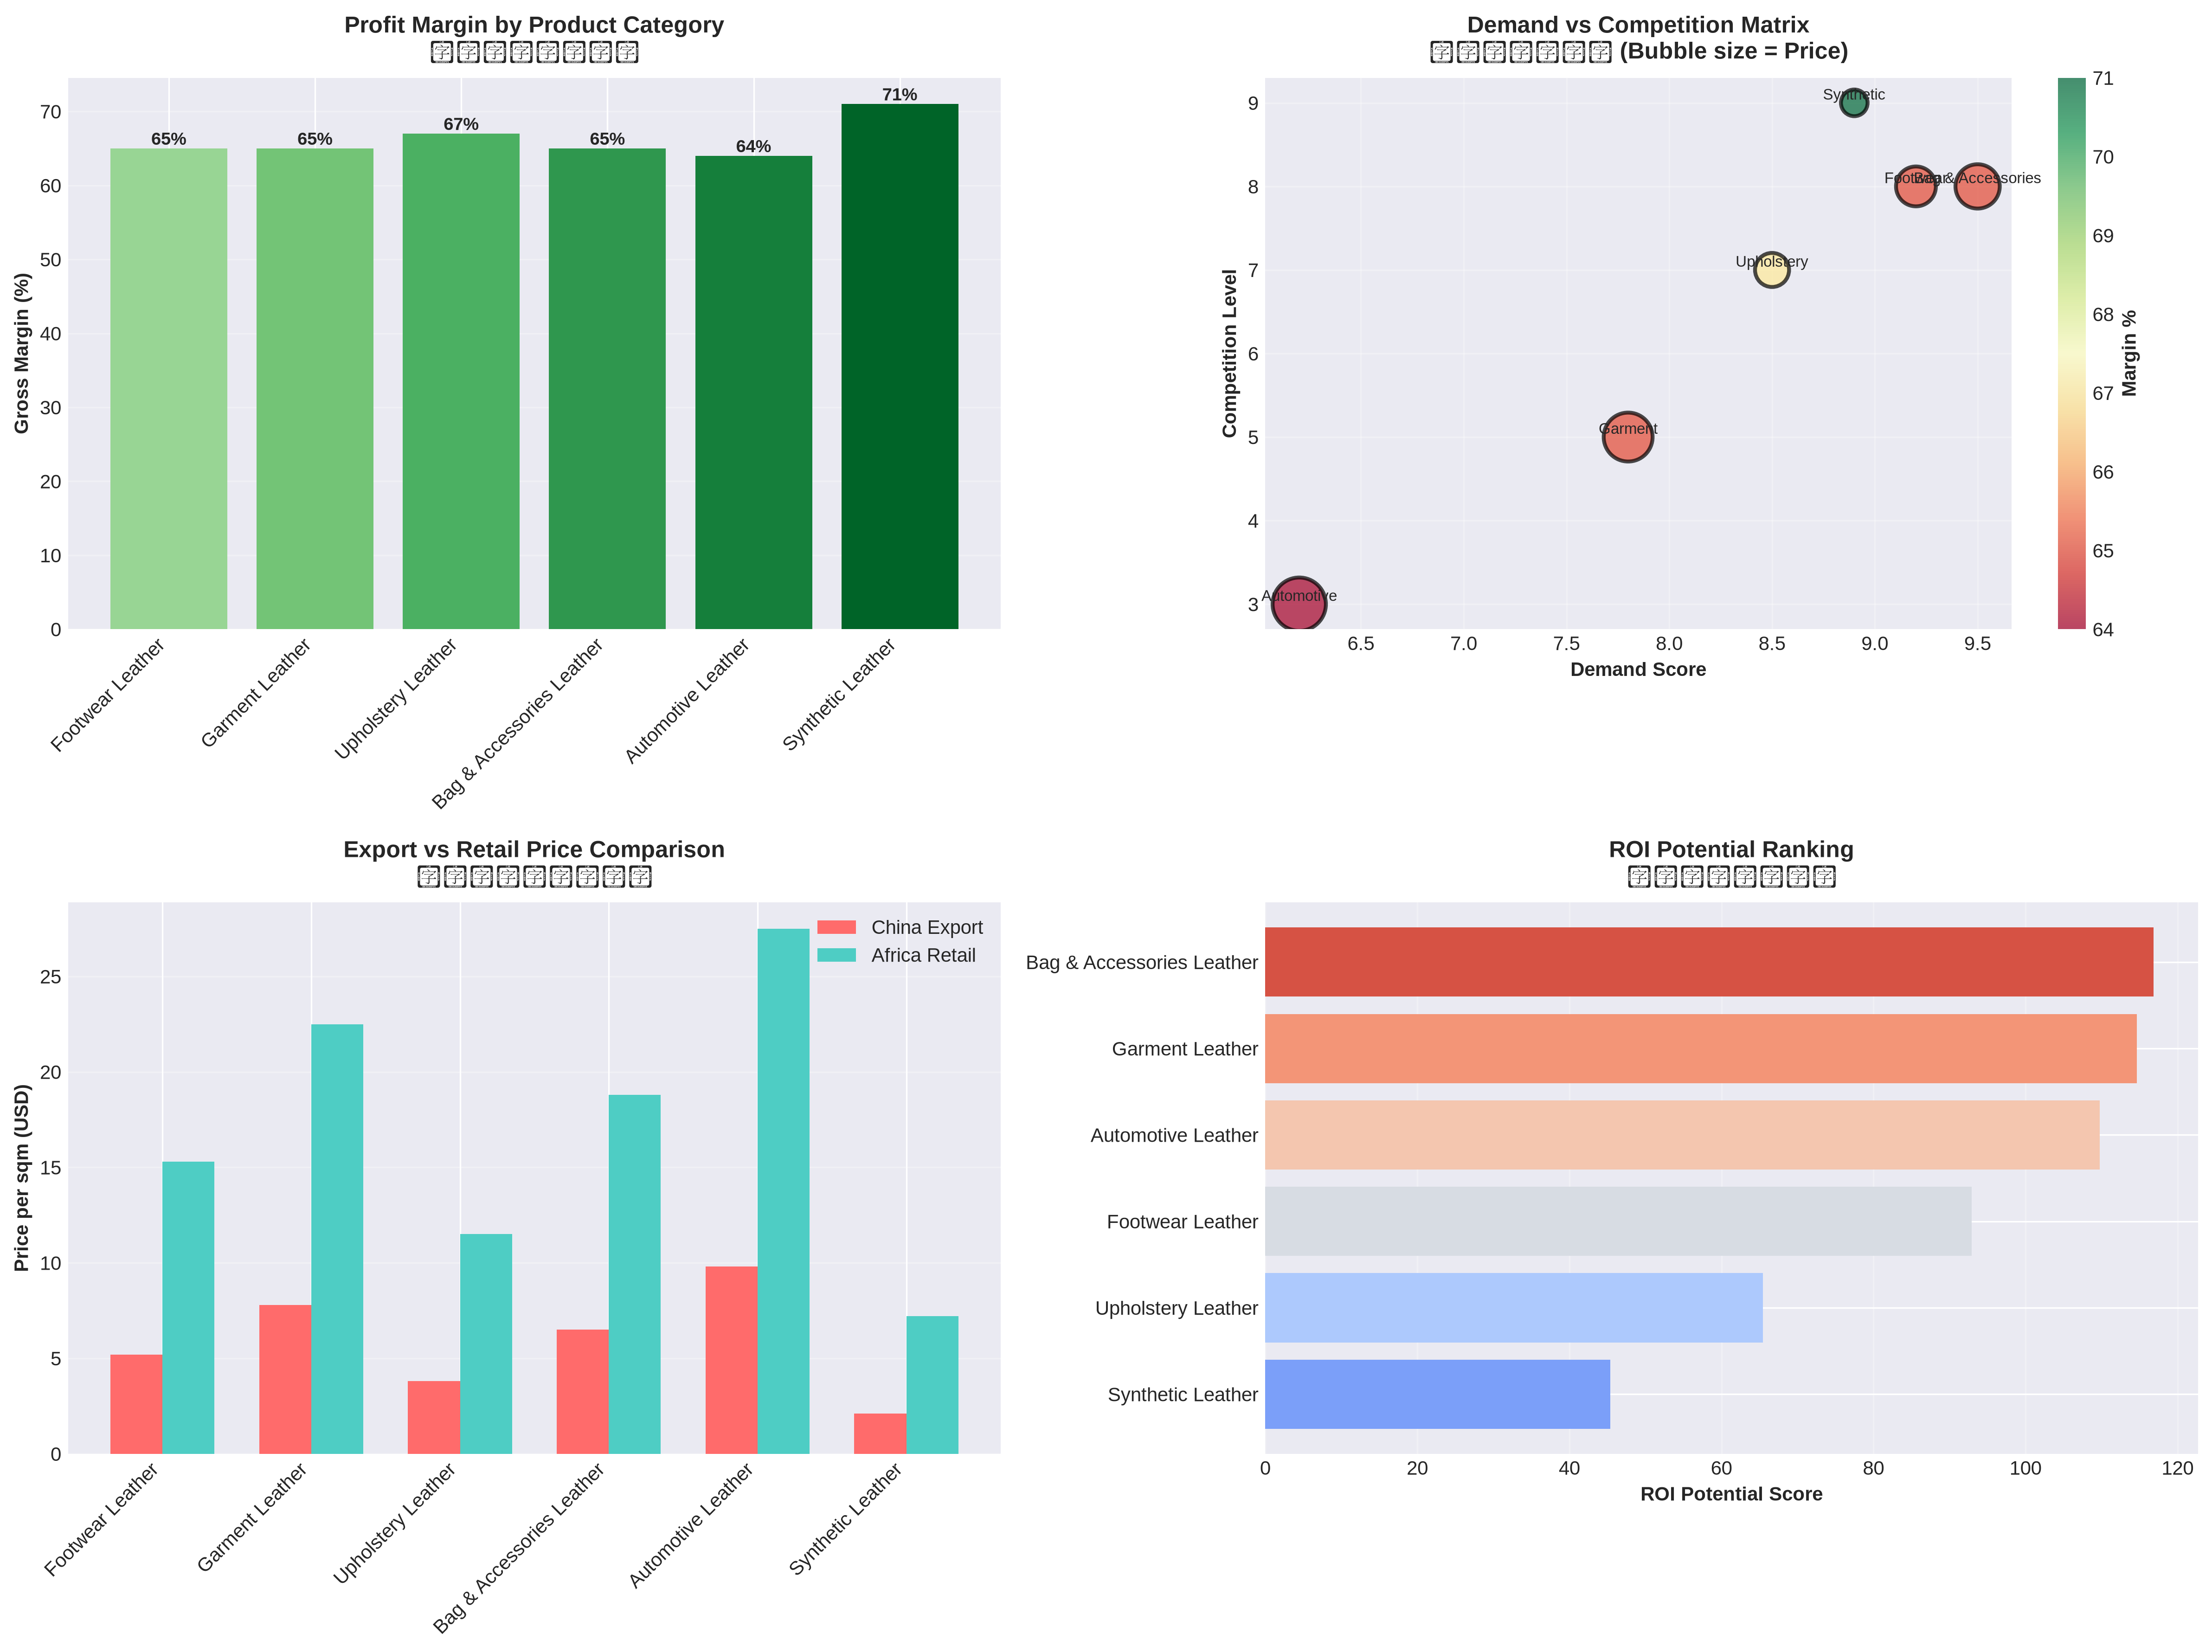
\includegraphics[width=0.95\textwidth]{figures/product_analysis.png}
\end{center}


\subsection*{English - Product Category Insights}
Six primary leather categories present varying margin and demand profiles:

\begin{enumerate}
    \item \textbf{Bag \& Accessories Leather} - Highest demand score (9.5/10), 65\% margin
    \item \textbf{Footwear Leather} - Strong demand (9.2/10), most competitive segment
    \item \textbf{Synthetic Leather} - Highest margin (71\%), very high competition
    \item \textbf{Garment Leather} - Premium pricing, requires high quality
    \item \textbf{Upholstery Leather} - Solid margins (67\%), medium competition
    \item \textbf{Automotive Leather} - Highest price point, specialized market
\end{enumerate}

\subsection*{Deutsch - Produktkategorien-Einblicke}
Sechs primäre Lederkategorien mit unterschiedlichen Margen- und Nachfrageprofilen.

\subsection*{Русский - Анализ категорий продукции}
Шесть основных категорий кожи с различной маржой и спросом.

\begin{CJK}{UTF8}{gbsn}
\subsection*{中文 - 产品类别洞察}
六个主要皮革类别具有不同的利润率和需求特征。
\end{CJK}

\newpage

%=============================================================================
\section{PESTEL Analysis / PESTEL-Analyse / PESTEL анализ / PESTEL分析}
%=============================================================================

\begin{center}
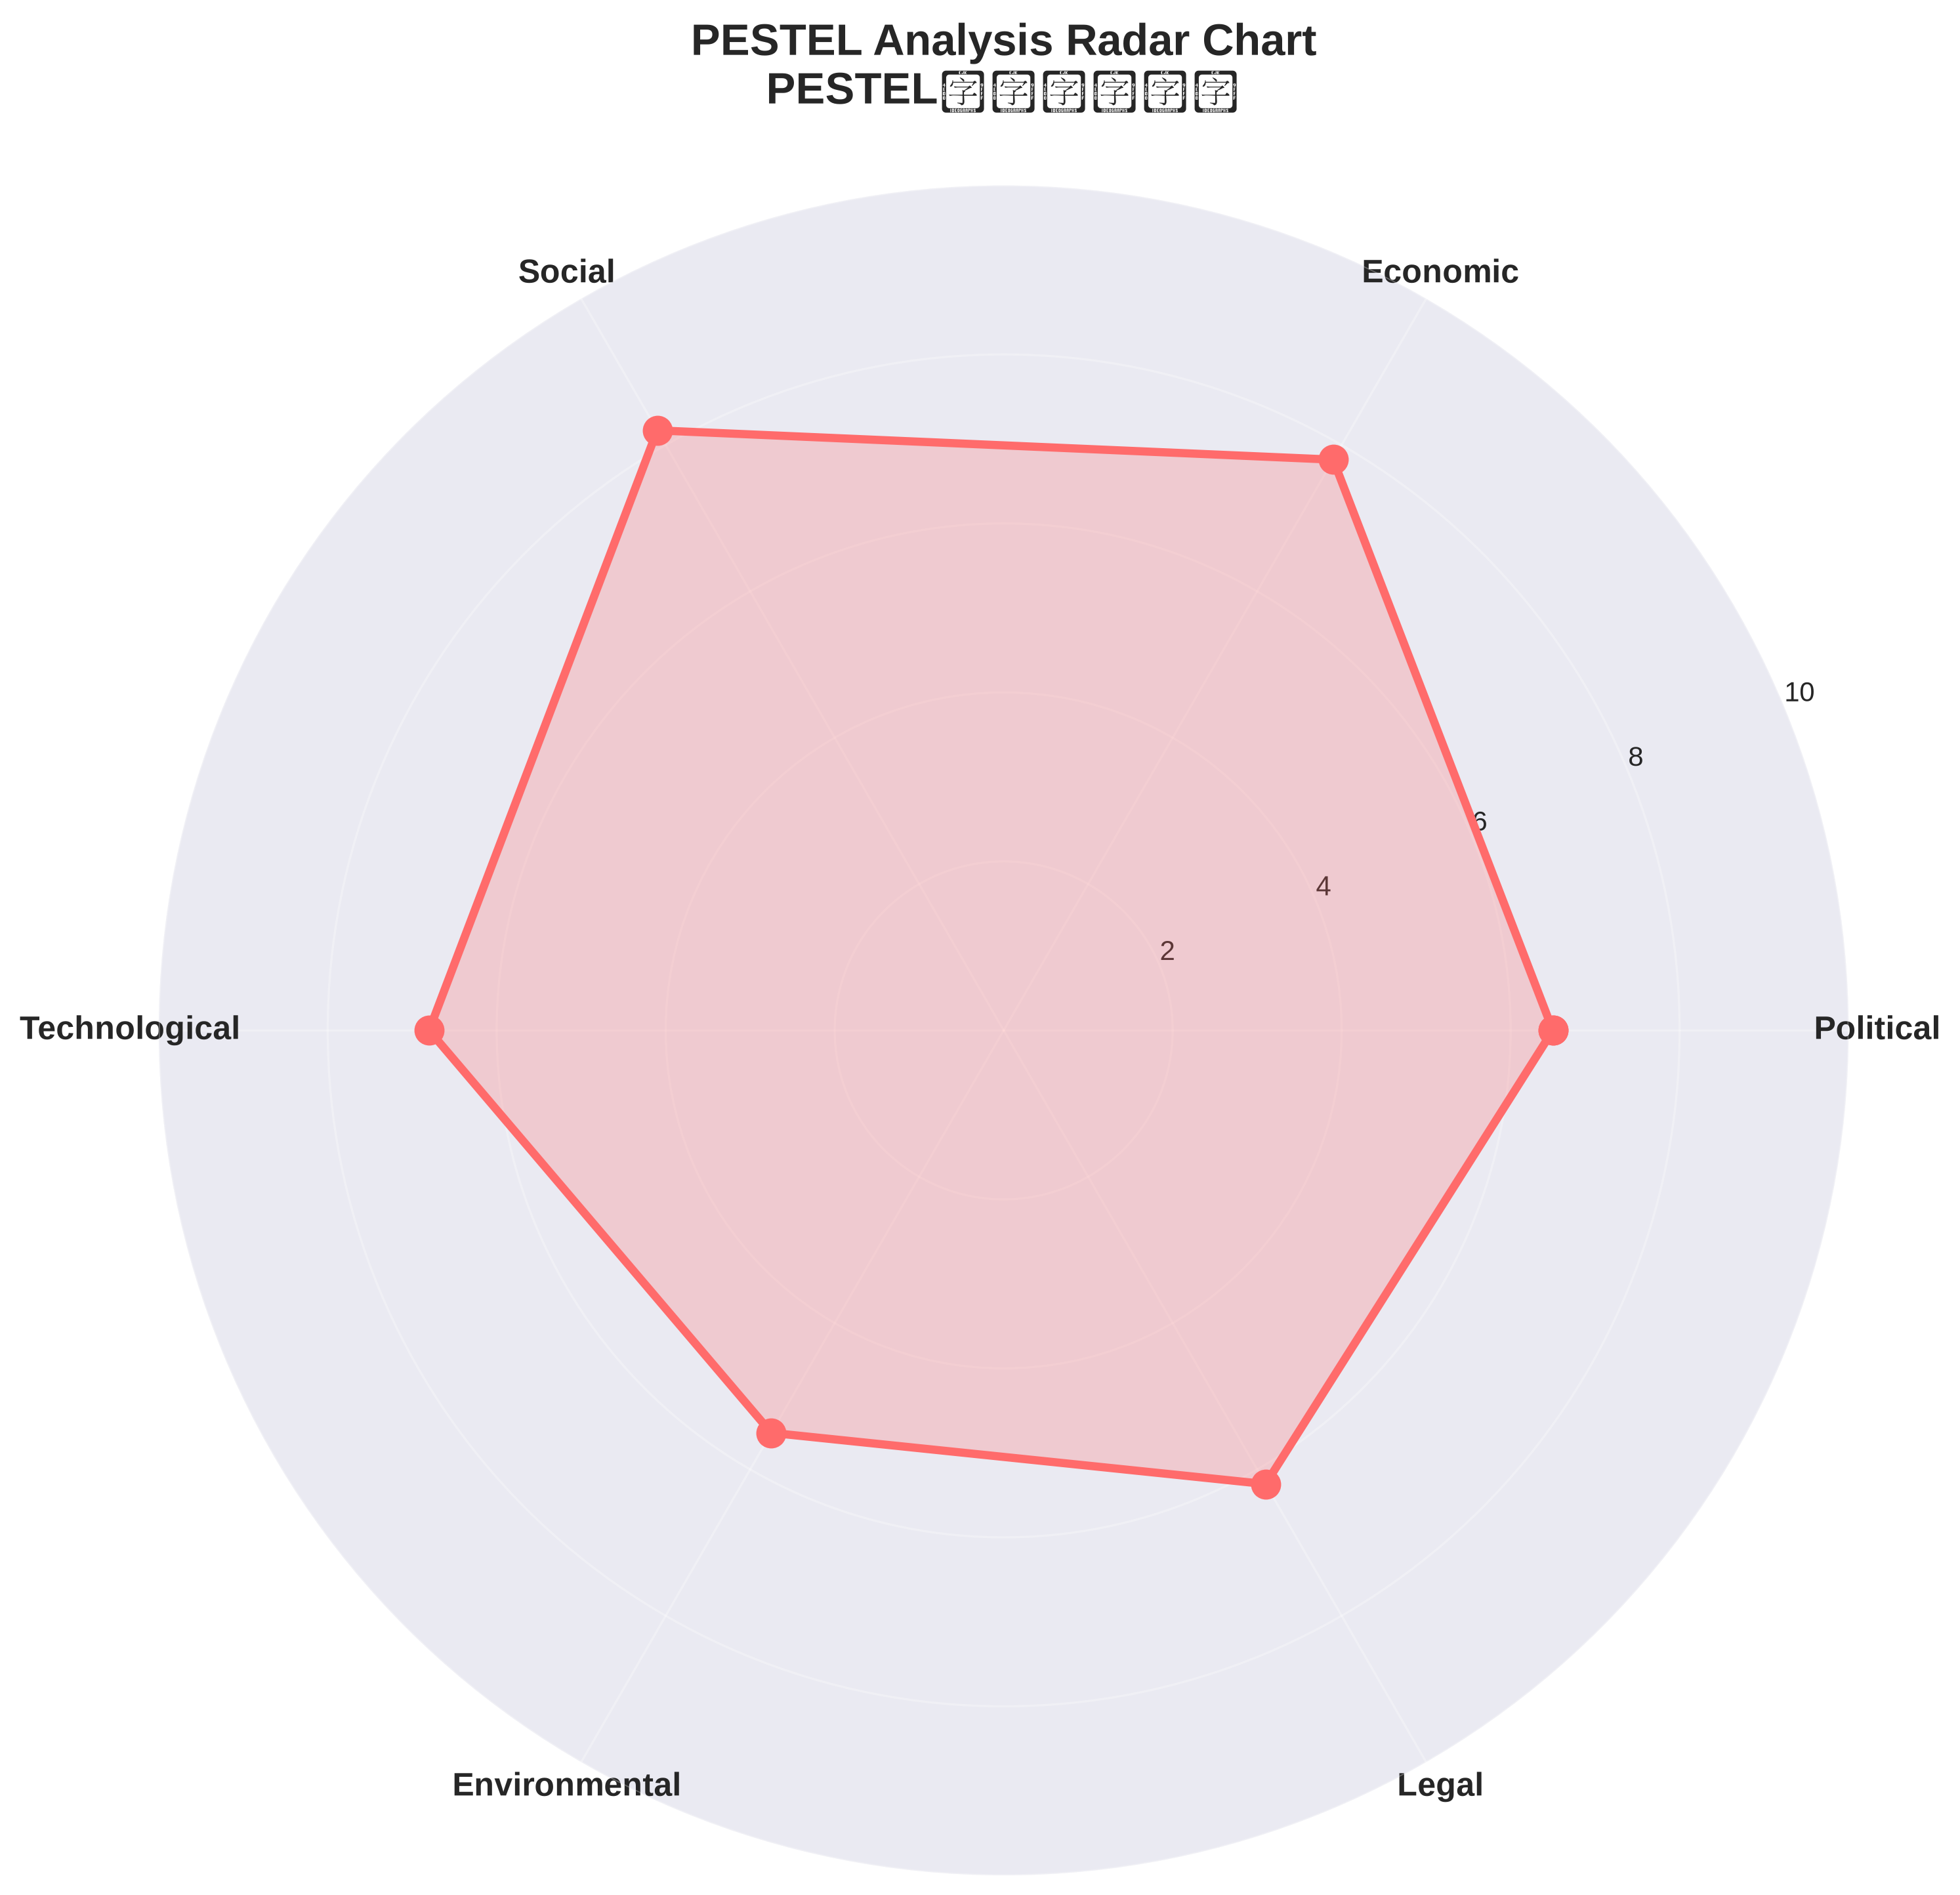
\includegraphics[width=0.7\textwidth]{figures/pestel_radar.png}
\end{center}

\subsection*{English - Macro Environment Assessment}

\textbf{Political (6.5/10):} China-Africa Forum and Belt \& Road Initiative strengthen trade relations. AfCFTA reduces intra-African barriers. Regional political instability remains a risk factor.

\textbf{Economic (7.8/10):} African middle class growing rapidly (300M+ by 2025). Leather import demand increasing 8-12\% annually. Chinese manufacturing offers 40-60\% cost advantage. Strong ROI potential confirmed.

\textbf{Social (8.2/10):} Urbanization driving consumption. Youth population (median age 19) seeking modern products. Status-driven consumption in emerging middle class. Preference for imported Chinese goods.

\textbf{Technological (6.8/10):} E-commerce penetration increasing. Mobile payment adoption (M-Pesa). Supply chain digitization improving. Limited quality preservation infrastructure.

\textbf{Environmental (5.5/10):} Increasing regulations on leather processing. Sustainability concerns. Water scarcity in tanning. Push for eco-friendly alternatives. Shipping carbon footprint.

\textbf{Legal (6.2/10):} Import duties vary (15-35\%). Customs complexity. Limited IP protection. Contract enforcement challenges. Need for local partnerships.


\newpage

%=============================================================================
\section{Risk Analysis / Risikoanalyse / Анализ рисков / 风险分析}
%=============================================================================

\begin{center}
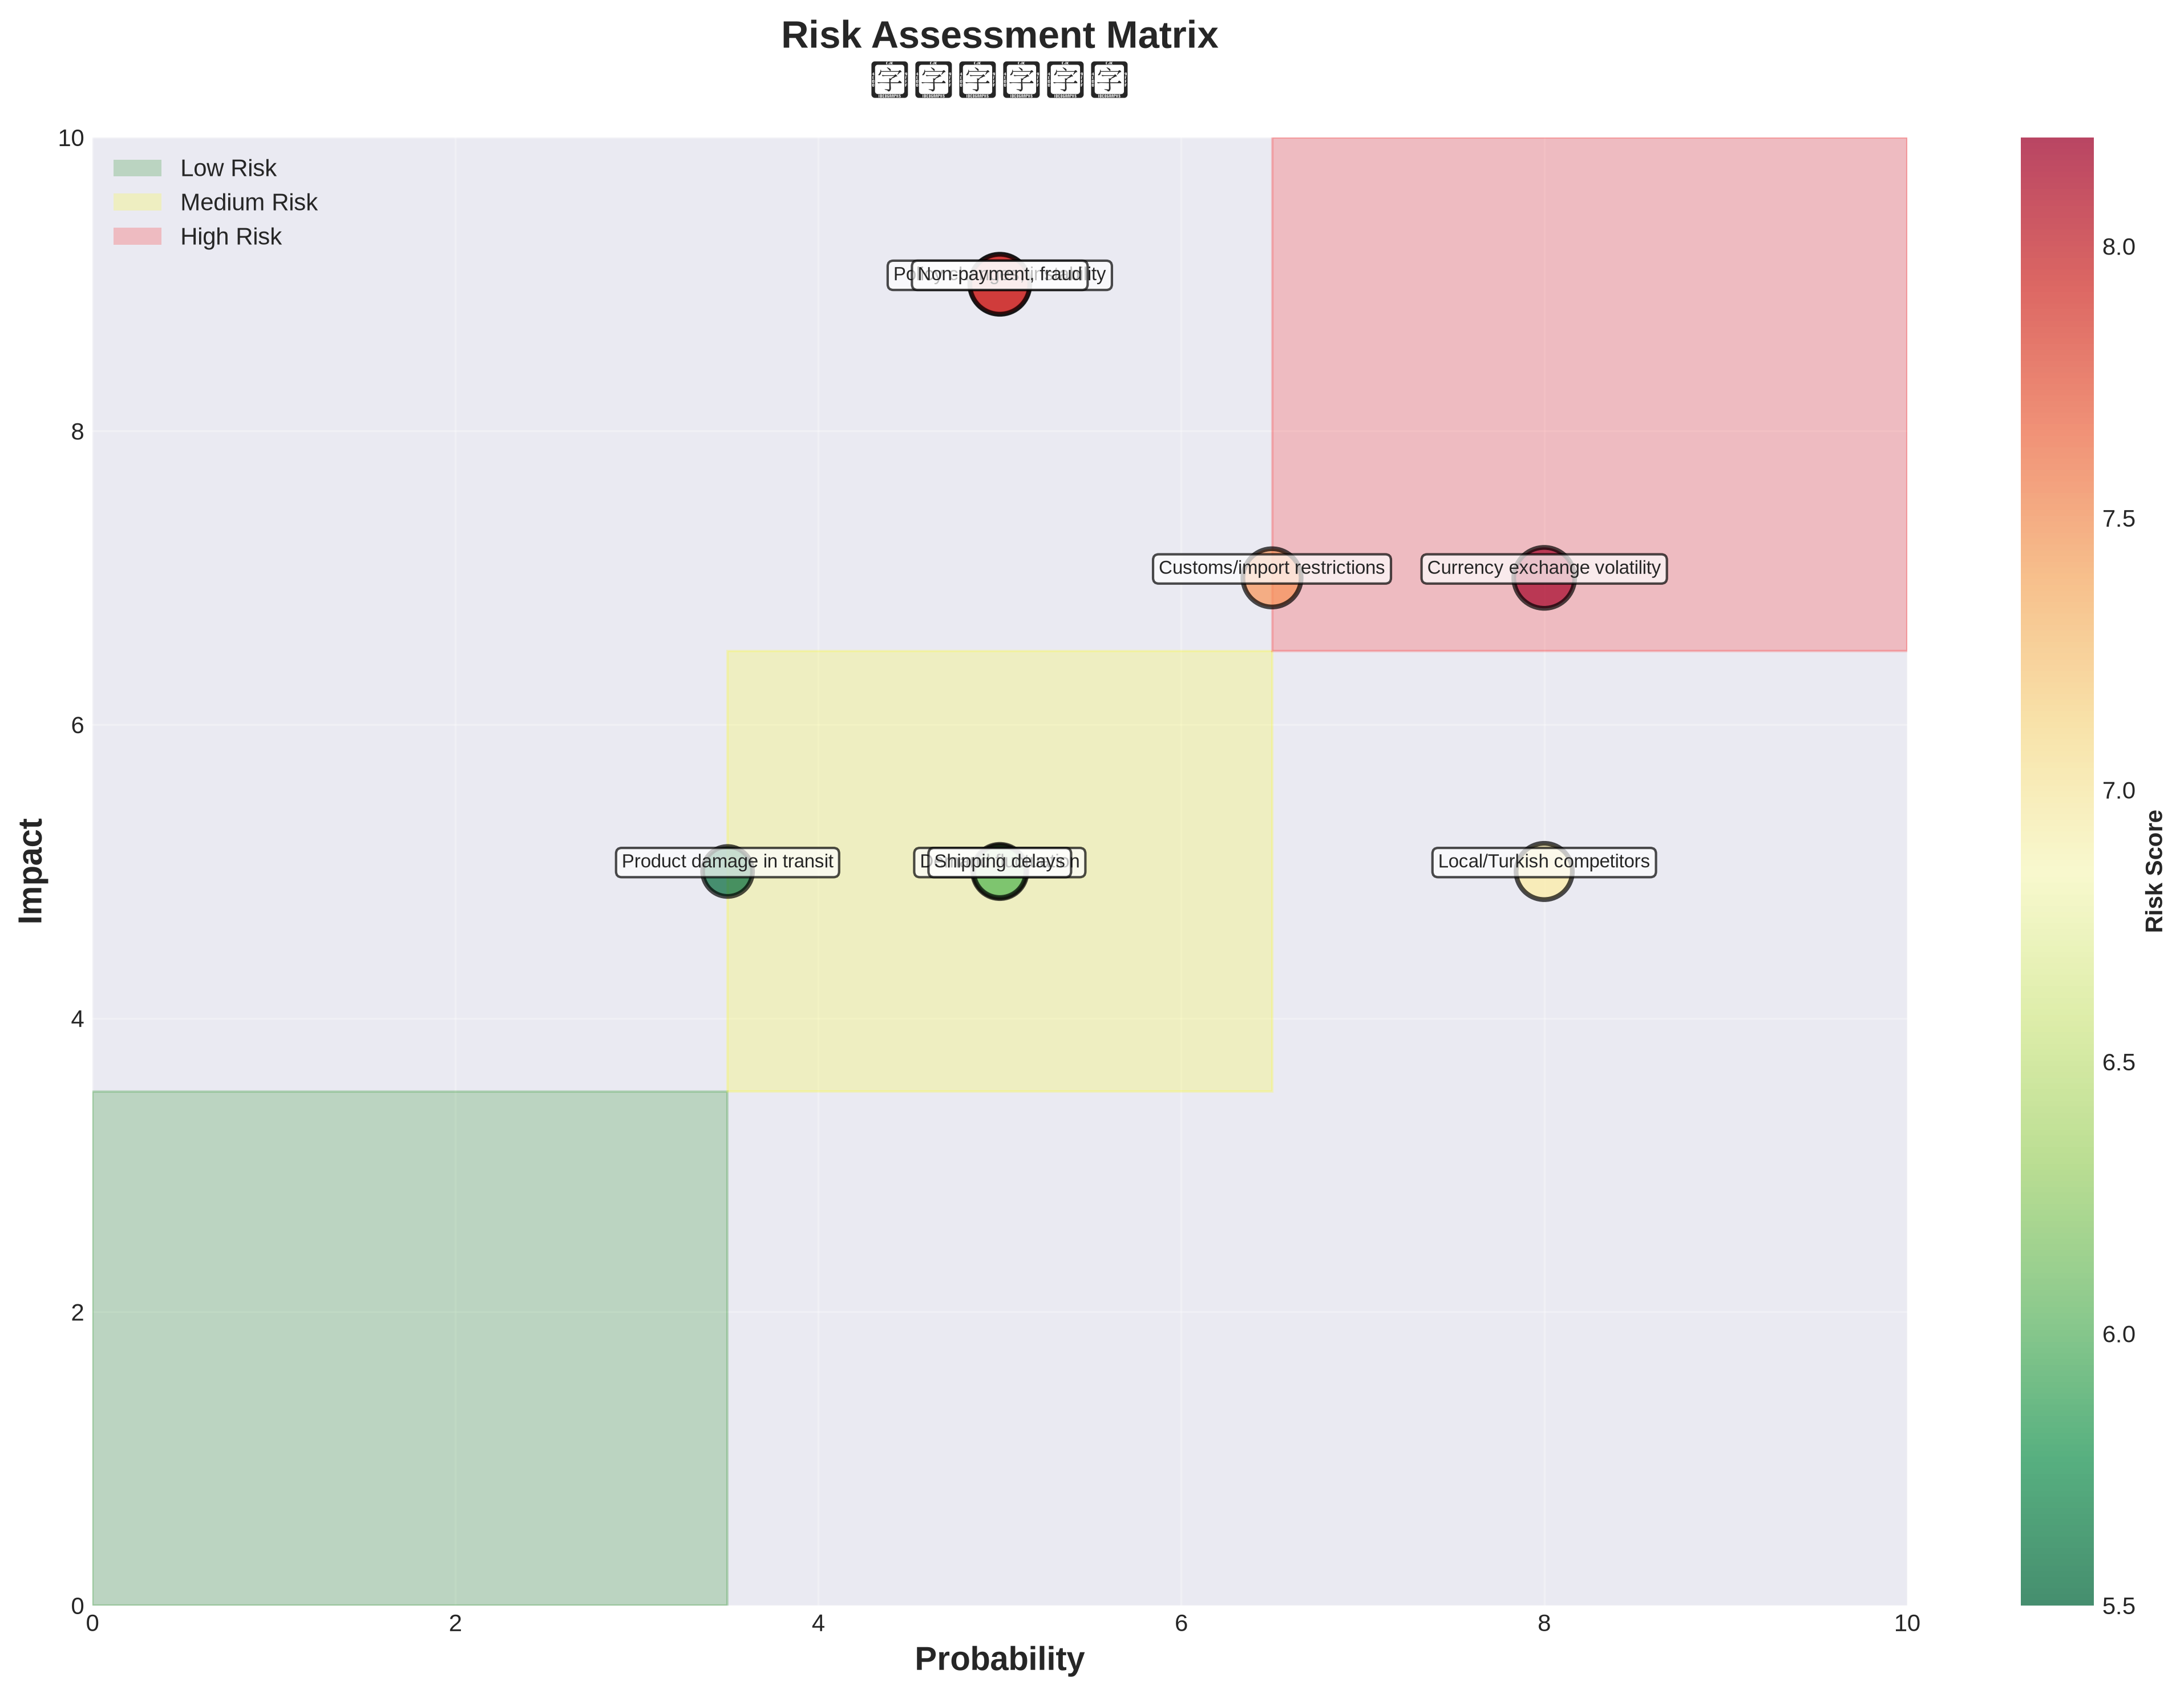
\includegraphics[width=0.95\textwidth]{figures/risk_matrix.png}
\end{center}

\subsection*{English - Key Risk Factors}

\textbf{High-Risk Items:}
\begin{itemize}
    \item Currency exchange volatility (Risk Score: 8.2) - \textit{Mitigation: Hedge FX, price in USD}
    \item Payment risk / fraud (Risk Score: 8.0) - \textit{Mitigation: LC/escrow, vetted partners}
    \item Political instability (Risk Score: 7.8) - \textit{Mitigation: Diversify countries}
    \item Customs restrictions (Risk Score: 7.5) - \textit{Mitigation: Local agents, compliance}
\end{itemize}

\textbf{Medium-Risk Items:}
\begin{itemize}
    \item Competition from Turkish/local suppliers (Risk Score: 7.0)
    \item Demand fluctuations (Risk Score: 6.5)
    \item Shipping delays (Risk Score: 6.0)
    \item Product damage in transit (Risk Score: 5.5)
\end{itemize}


\newpage

%=============================================================================
\section{Strategic Recommendations / Strategische Empfehlungen / Стратегические рекомендации / 战略建议}
%=============================================================================

\subsection*{English}

\textbf{1. Market Entry Strategy}
\begin{itemize}
    \item \textbf{Phase 1:} Start with South Africa and Nigeria (largest markets, established logistics)
    \item \textbf{Phase 2:} Expand to Kenya and Ghana (high growth rates)
    \item \textbf{Phase 3:} Enter Ethiopia and Tanzania (emerging markets, lower competition)
\end{itemize}

\textbf{2. Product Mix Optimization}
\begin{itemize}
    \item Focus 60\% on Footwear \& Bag Leather (high demand, good margins)
    \item Allocate 30\% to Upholstery Leather (stable demand)
    \item Reserve 10\% for Synthetic Leather (volume play)
\end{itemize}

\textbf{3. Risk Management}
\begin{itemize}
    \item Establish LC (Letter of Credit) payment terms for first 3-6 months
    \item Partner with local distributors who have existing networks
    \item Maintain 2-3 week inventory buffer at destination
    \item Hedge 70-80\% of FX exposure on shipments $>$ \$50,000
\end{itemize}

\textbf{4. Logistics Optimization}
\begin{itemize}
    \item Consolidate shipments to achieve 95\%+ container utilization
    \item Negotiate volume discounts with shipping lines (target: 15-20\% reduction after 10 containers)
    \item Utilize bonded warehouses at destination ports to defer customs duties
    \item Implement GPS tracking and marine insurance for all shipments
\end{itemize}

\textbf{5. Competitive Positioning}
\begin{itemize}
    \item Price 10-15\% below Turkish leather imports
    \item Emphasize consistent quality and supply reliability
    \item Offer flexible payment terms after relationship establishment
    \item Provide technical support and after-sales service
\end{itemize}

\subsection*{Deutsch - Wichtigste Empfehlungen}
1. Einstieg über Südafrika und Nigeria\\
2. Fokus auf Schuh- und Taschenleder\\
3. LC-Zahlungsbedingungen etablieren\\
4. Lokale Partnerschaften aufbauen

\subsection*{Русский - Ключевые рекомендации}
1. Выход на рынок через ЮАР и Нигерию\\
2. Фокус на обувной и сумочной коже\\
3. Установить условия оплаты по LC\\
4. Создать местные партнерства

\begin{CJK}{UTF8}{gbsn}
\subsection*{中文 - 关键建议}
1. 通过南非和尼日利亚进入市场\\
2. 专注于鞋类和箱包皮革\\
3. 建立信用证支付条款\\
4. 建立本地合作伙伴关系
\end{CJK}

\newpage

%=============================================================================
\section{Financial Projections / Finanzprognosen / Финансовые прогнозы / 财务预测}
%=============================================================================

\subsection*{English - 12-Month Projection}

\textbf{Scenario: Conservative (1 container per month)}
\begin{itemize}
    \item Monthly Revenue: \$130,000 - \$140,000
    \item Monthly Gross Profit: \$73,700 - \$88,550
    \item Annual Gross Profit: \textbf{\$884,400 - \$1,062,600}
    \item Required Working Capital: \$52,700 (recurring)
\end{itemize}

\textbf{Scenario: Moderate (2 containers per month)}
\begin{itemize}
    \item Monthly Revenue: \$260,000 - \$280,000
    \item Annual Gross Profit: \textbf{\$1.77M - \$2.13M}
    \item Required Working Capital: \$105,400
\end{itemize}

\textbf{Scenario: Aggressive (4 containers per month)}
\begin{itemize}
    \item Monthly Revenue: \$520,000 - \$560,000
    \item Annual Gross Profit: \textbf{\$3.54M - \$4.25M}
    \item Required Working Capital: \$210,800
\end{itemize}

\textit{Note: Projections assume consistent demand, stable pricing, and successful payment collection.}


\newpage

%=============================================================================
\section{Data Appendix / Datenanhang / Приложение данных / 数据附录}
%=============================================================================

\subsection{Market Data Summary / Marktdaten / Рыночные данные / 市场数据}

\begin{longtable}{lrrr}
\toprule
\textbf{Country} & \textbf{Market Size (\$M)} & \textbf{Growth (\%)} & \textbf{Chinese Share (\%)} \\
\midrule
Nigeria & 580 & 8.9 & 38 \\
South Africa & 920 & 6.2 & 29 \\
Kenya & 340 & 10.7 & 44 \\
Ghana & 210 & 9.5 & 41 \\
Egypt & 1250 & 7.1 & 35 \\
Morocco & 680 & 5.8 & 26 \\
Ethiopia & 280 & 12.5 & 52 \\
Tanzania & 195 & 9.8 & 47 \\
\bottomrule
\end{longtable}

\subsection{Container Economics by Route / Container-Ökonomie / Экономика контейнеров / 集装箱经济}

\begin{longtable}{lrrr}
\toprule
\textbf{Route} & \textbf{Investment (\$)} & \textbf{Revenue (\$)} & \textbf{ROI (\%)} \\
\midrule
Nigeria & 52700 & 130050 & 147 \\
Kenya & 52100 & 125800 & 141 \\
South Africa & 51700 & 140250 & 171 \\
\bottomrule
\end{longtable}


\newpage

%=============================================================================
\section{Conclusion / Fazit / Заключение / 结论}
%=============================================================================

\subsection*{English}
The Africa leather trade presents a \textbf{compelling investment opportunity} with:
\begin{itemize}
    \item Proven ROI of 141-171\% per shipment
    \item Rapid payback period ($<$1 month)
    \item Growing market demand (8-12\% annually)
    \item Established logistics infrastructure
    \item Strong competitive positioning from Chinese manufacturing
\end{itemize}

\textbf{Success factors:} Local partnerships, proper risk management, product quality consistency, and market-appropriate pricing strategy.

\textbf{Next steps:} Identify reliable Chinese leather suppliers, establish relationships with African distributors, secure initial LC payment terms, and execute pilot shipment to test market response.

\subsection*{Deutsch}
Der afrikanische Lederhandel bietet eine \textbf{überzeugende Investitionsmöglichkeit} mit nachgewiesener Rendite von 141-171\% pro Lieferung.

\subsection*{Русский}
Африканская кожаная торговля представляет \textbf{привлекательную инвестиционную возможность} с доказанной рентабельностью 141-171\% на отгрузку.

\begin{CJK}{UTF8}{gbsn}
\subsection*{中文}
非洲皮革贸易提供了一个\textbf{引人注目的投资机会}，每次运输的投资回报率为141-171\%。
\end{CJK}

\vspace{2cm}

\begin{center}
\textbf{\Large --- End of Report / Ende des Berichts / Конец отчёта / 报告结束 ---}
\end{center}

\end{document}
